% LaTeX Language and campus name and format package
\documentclass[es,gi]{ifirak}\usepackage[]{graphicx}\usepackage[]{color}
%% maxwidth is the original width if it is less than linewidth
%% otherwise use linewidth (to make sure the graphics do not exceed the margin)
\makeatletter
\def\maxwidth{ %
  \ifdim\Gin@nat@width>\linewidth
    \linewidth
  \else
    \Gin@nat@width
  \fi
}
\makeatother

\definecolor{fgcolor}{rgb}{0.345, 0.345, 0.345}
\newcommand{\hlnum}[1]{\textcolor[rgb]{0.686,0.059,0.569}{#1}}%
\newcommand{\hlstr}[1]{\textcolor[rgb]{0.192,0.494,0.8}{#1}}%
\newcommand{\hlcom}[1]{\textcolor[rgb]{0.678,0.584,0.686}{\textit{#1}}}%
\newcommand{\hlopt}[1]{\textcolor[rgb]{0,0,0}{#1}}%
\newcommand{\hlstd}[1]{\textcolor[rgb]{0.345,0.345,0.345}{#1}}%
\newcommand{\hlkwa}[1]{\textcolor[rgb]{0.161,0.373,0.58}{\textbf{#1}}}%
\newcommand{\hlkwb}[1]{\textcolor[rgb]{0.69,0.353,0.396}{#1}}%
\newcommand{\hlkwc}[1]{\textcolor[rgb]{0.333,0.667,0.333}{#1}}%
\newcommand{\hlkwd}[1]{\textcolor[rgb]{0.737,0.353,0.396}{\textbf{#1}}}%
\let\hlipl\hlkwb

\usepackage{framed}
\makeatletter
\newenvironment{kframe}{%
 \def\at@end@of@kframe{}%
 \ifinner\ifhmode%
  \def\at@end@of@kframe{\end{minipage}}%
  \begin{minipage}{\columnwidth}%
 \fi\fi%
 \def\FrameCommand##1{\hskip\@totalleftmargin \hskip-\fboxsep
 \colorbox{shadecolor}{##1}\hskip-\fboxsep
     % There is no \\@totalrightmargin, so:
     \hskip-\linewidth \hskip-\@totalleftmargin \hskip\columnwidth}%
 \MakeFramed {\advance\hsize-\width
   \@totalleftmargin\z@ \linewidth\hsize
   \@setminipage}}%
 {\par\unskip\endMakeFramed%
 \at@end@of@kframe}
\makeatother

\definecolor{shadecolor}{rgb}{.97, .97, .97}
\definecolor{messagecolor}{rgb}{0, 0, 0}
\definecolor{warningcolor}{rgb}{1, 0, 1}
\definecolor{errorcolor}{rgb}{1, 0, 0}
\newenvironment{knitrout}{}{} % an empty environment to be redefined in TeX

\usepackage{alltt}

% ERABILIKO DIREN PAKETEAK %

% listings pakage is for code formating
\usepackage{listings}
% Paquete for acents and other special characters
% It is not necesary to use all this packages add or remove those you are interested on
\usepackage[utf8]{inputenc}
\usepackage{colortbl}
\usepackage[table]{xcolor}
\usepackage{graphicx}
\usepackage{wrapfig}
\usepackage{amsfonts}
\usepackage{makeidx}
\usepackage{adjustbox}

% Definition of colors
\definecolor{darkgreen}{rgb}{0,0.5,0}
\definecolor{lightgray}{rgb}{0.95,0.95,0.95}
\definecolor{gray}{rgb}{0.85,0.85,0.85}
\definecolor{white}{rgb}{1,1,1}
\definecolor{purple}{rgb}{0.51,0,0.25}
\definecolor{orange}{rgb}{0.255,0.178,0.102}
%Definition of style for code
\lstdefinestyle{customc}{
	belowcaptionskip=1\baselineskip,
	breaklines=true,
	tabsize=4,
	language=C,
	showstringspaces=false,
	basicstyle=\footnotesize\ttfamily,
	keywordstyle=\bfseries\color{darkgreen},
	commentstyle=\itshape\color{purple},
	identifierstyle=\color{blue},
	stringstyle=\color{orange},
	backgroundcolor=\color{lightgray},
}
\lstset{language=C,escapechar=@,style=customc}
\DeclareMathSizes{10}{10}{10}{10}
%\lstset{language=C++,
	%	basicstyle=\scriptsize\ttfamily,
	%	keywordstyle=\color{darkgreen}\bfseries,
	%	identifierstyle=\color{black},
	%	commentstyle=\color{gray}, 
	%	stringstyle=\ttfamily,
	%	showstringspaces=false,
	%	tabsize=2,
%	\textit{K}(\textit{m}, \textit{j}) = max \{ \textit{K}(\textit{m} - \textit{m_{j}}, \textit{j} - 1) + \textit{v_{j}} , \textit{K}(\textit{m}, \textit{j} - 1) \}
	%	backgroundcolor=\color{lightgray}}
%par(pch=22, col="black", mfrow = c(2,1))
\IfFileExists{upquote.sty}{\usepackage{upquote}}{}
\begin{document}

% Course year
\ikasturtea{2018 - 2019}
% Subject or course name
\irakasgaia{Visión por Computador}
% Title
\title{Desafíos 2, 3 y 4}
% Name of Author
\author{Mikel Dalmau}

\maketitle



%\section{Código}

\section{Enunciados}

\subsection{Desafío 2}
\paragraph{}
El objetivo es crear una tabla de caraceristicas geometricas de las imagenes utilizando la herramienta de matlab regionprops.

\begin{itemize}
\item[•] ¿es factible compararlos y distinguirlos?
\item[•] ¿que caracteristicas parecen ser más distitivas?
\end{itemize}

\subsection{Desafío 3}
\paragraph{}
El objetivo es crear una tabla de caraceristicas geometricas de las imagenes corrigiendo los problemas que plantean las ditintas orientaciones utilizando las herramientas de matlab regionprops, imrotate.

\subsection{Desafío 4}
\paragraph{}
El objetivo es asegurar que todas y cada una de las imágenes solo tienen un componente sin agujeros.

\section{Procesado de las imágenes}
\paragraph{•}
\subsection{Binarizar la imagen}

\subsection{Computar las propiedades}

\subsection{Rotar las imágenes}

\subsection{Procesos Previos a la binarización}

\section{Clasificación}

\begin{figure}[hbtp]
\centering
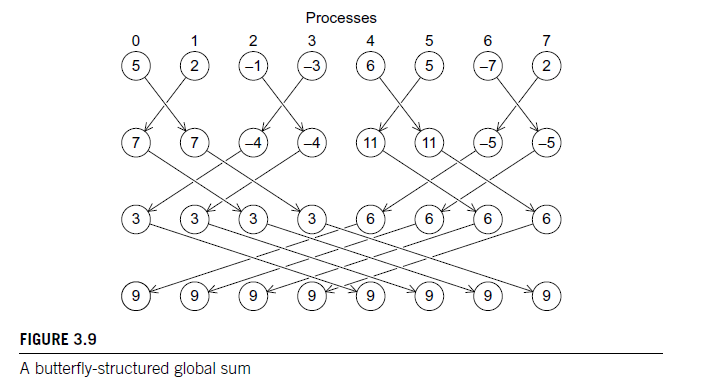
\includegraphics[scale=0.5]{Butterfly.png}
\caption{Martillo1 Original}
\end{figure}

\begin{thebibliography}{arauak}
	
	\bibitem[1]{key-1} Matlab official documentation:\textit{es.mathworks.com}
	
	\bibitem[2]{key-2} 
\end{thebibliography}


\end{document}
